Nesta seção, apresentamos e discutimos os resultados obtidos com a aplicação dos quatro algoritmos de agrupamento (KMeans, Fuzzy C-Means, Gustafson-Kessel e Agglomerativo) nos conjuntos de dados Adult e Dry Bean. São analisadas as métricas quantitativas, as visualizações e as principais observações para cada cenário, destacando as vantagens, limitações e particularidades de cada abordagem em contextos binário e multiclasse.

\subsection{Bases de Dados e Pré-processamento}

Neste trabalho, utilizamos os conjuntos de dados \textbf{Adult} (Census Income) e \textbf{Dry Bean}, ambos amplamente empregados em tarefas de classificação e agrupamento. Para garantir a comparabilidade entre os métodos, em ambos os casos foi realizado o seguinte pré-processamento: todas as variáveis categóricas foram transformadas em representações numéricas, os atributos foram normalizados e os dados foram divididos de forma estratificada em 70\% para treinamento e 30\% para teste. No caso do conjunto Adult, devido ao desbalanceamento entre as classes, aplicou-se também uma técnica de balanceamento (como oversampling) para garantir uma distribuição mais equitativa entre as categorias de renda.

\textbf{Adult:} O conjunto Adult contém aproximadamente 48 mil amostras de indivíduos adultos dos Estados Unidos, com atributos demográficos e socioeconômicos, distribuídos em duas classes principais (renda >50K e <=50K). Os atributos incluem variáveis numéricas e categóricas, exigindo codificação e normalização cuidadosas. O balanceamento foi fundamental para evitar viés nos resultados devido à predominância de uma das classes.

\textbf{Dry Bean:} O conjunto Dry Bean é composto por mais de 13 mil amostras de feijões secos de sete diferentes cultivares, com atributos morfológicos extraídos de imagens. Todos os atributos são numéricos, facilitando a aplicação direta das técnicas de normalização. A distribuição das classes é naturalmente mais equilibrada, não sendo necessário aplicar técnicas adicionais de balanceamento. Essa preparação garante que os métodos de agrupamento possam explorar de forma justa as relações entre as amostras e as classes reais.

\subsection{Seleção do Número de Clusters: Método do Cotovelo}

Antes de aplicar os algoritmos de agrupamento, foi utilizado o método do cotovelo para determinar o número ideal de clusters em cada conjunto de dados. O método consiste em executar o KMeans para diferentes valores de $k$ e calcular a soma dos erros quadráticos dentro dos clusters (inertia). O ponto em que a redução do erro começa a diminuir significativamente indica o número adequado de clusters, conhecido como "cotovelo" da curva. Esse valor de $k$ foi então utilizado como referência para todos os algoritmos testados, garantindo uma comparação justa entre os métodos.

No dataset Adult, o método do cotovelo sugeriu a utilização de 2 clusters, alinhando-se ao número de classes reais (renda >50K e <=50K). Já no Dry Bean, o cotovelo foi observado em $k=7$, correspondente ao número de cultivares presentes no conjunto.

As Figuras~\ref{fig:elbow_adult} e \ref{fig:elbow_drybean} ilustram as curvas do método do cotovelo para os dois datasets.

\begin{figure}[ht]
    \centering
    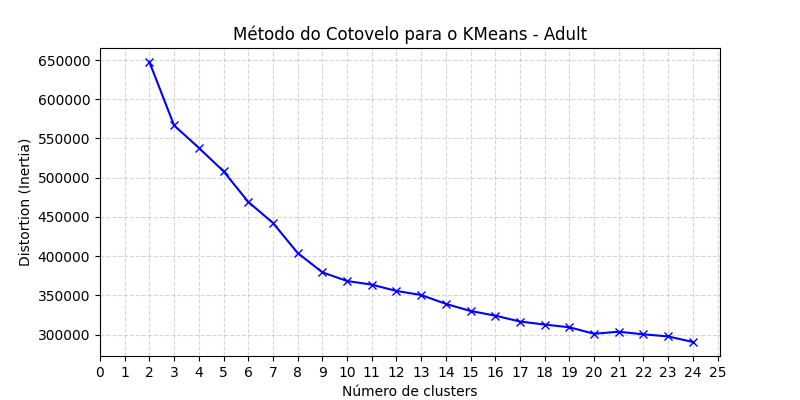
\includegraphics[width=0.8\linewidth]{../src/img/kmeans_adult_elbow.png}
    \caption{Curva do método do cotovelo para o dataset Adult.}
    \label{fig:elbow_adult}
\end{figure}

\begin{figure}[ht]
    \centering
    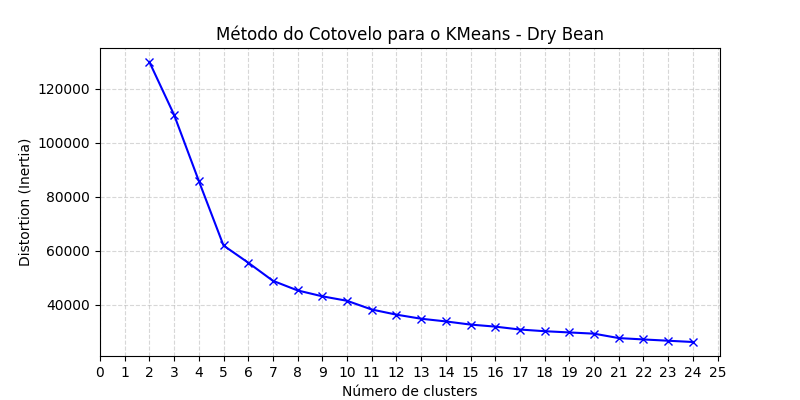
\includegraphics[width=0.8\linewidth]{../src/img/kmeans_drybean_elbow.png}
    \caption{Curva do método do cotovelo para o dataset Dry Bean.}
    \label{fig:elbow_drybean}
\end{figure}

\textbf{Setup de Teste:}
\begin{itemize}
    \item \textbf{Divisão dos dados:} 70\% para treinamento e 30\% para teste, com estratificação das classes.
    \item \textbf{Pré-processamento:} Codificação numérica das variáveis categóricas (quando presentes) e normalização dos atributos.
    \item \textbf{Balanceamento:} No Adult, foi realizado oversampling para igualar as classes; no Dry Bean, não foi necessário devido ao equilíbrio natural das classes.
    \item \textbf{Seleção do número de clusters:} Adult: 2 clusters (duas classes); Dry Bean: 7 clusters (sete classes), conforme sugerido pelo método do cotovelo.
    \item \textbf{Execuções:} 30 repetições com diferentes sementes para garantir robustez estatística dos resultados.
    \item \textbf{Parâmetros do algoritmo:} (Descreva aqui os parâmetros específicos do algoritmo, como grau de fuzzificação para Fuzzy C-Means, matriz de covariância para Gustafson-Kessel, etc.)
\end{itemize}


\subsection{KMeans}

O algoritmo KMeans foi aplicado de forma supervisionada tanto ao conjunto de dados Adult (balanceado) quanto ao Dry Bean, permitindo comparar o desempenho do método em cenários binário e multiclasse.



\textbf{Resultados:}

\textbf{Adult (balanceado):}
\begin{itemize}
    \item \textbf{Acurácia média:} (preencher valor)
    \item \textbf{Precisão média:} (preencher valor)
    \item \textbf{Recall médio:} (preencher valor)
    \item \textbf{Especificidade média:} (preencher valor)
    \item \textbf{F1-score médio:} (preencher valor)
\end{itemize}
As Figuras~\ref{fig:kmeans_adult_acc_repeticoes}, \ref{fig:kmeans_adult_mse_repeticoes} e \ref{fig:kmeans_adult_cm_media} ilustram a estabilidade da acurácia, o erro médio quadrático e a matriz de confusão média, respectivamente.

\begin{figure}[ht]
    \centering
    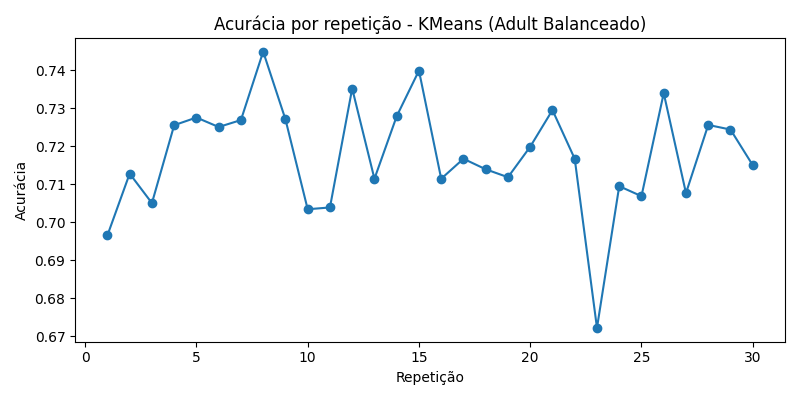
\includegraphics[width=0.9\linewidth]{../src/img/kmeans_adult_balance_accuracy_repetitions.png}
    \caption{Acurácia por repetição do KMeans no Adult balanceado.}
    \label{fig:kmeans_adult_acc_repeticoes}
\end{figure}

\begin{figure}[ht]
    \centering
    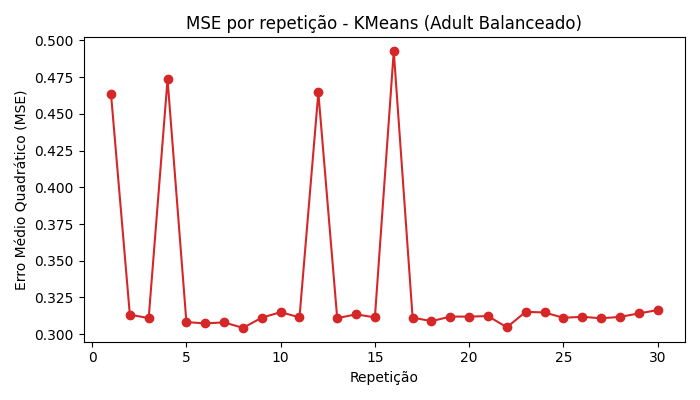
\includegraphics[width=0.9\linewidth]{../src/img/kmeans_adult_balance_mse_repetitions.png}
    \caption{Erro médio quadrático (MSE) por repetição no Adult balanceado.}
    \label{fig:kmeans_adult_mse_repeticoes}
\end{figure}

\begin{figure}[ht]
    \centering
    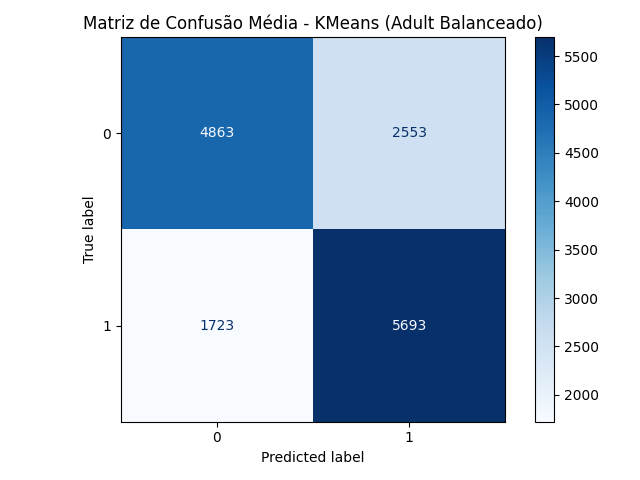
\includegraphics[width=0.9\linewidth]{../src/img/kmeans_adult_balance_confusion_matrix_media.png}
    \caption{Matriz de confusão média das execuções no Adult balanceado.}
    \label{fig:kmeans_adult_cm_media}
\end{figure}

\textbf{Dry Bean:}
\begin{itemize}
    \item \textbf{Acurácia média:} (preencher valor)
    \item \textbf{Precisão média:} (preencher valor)
    \item \textbf{Recall médio:} (preencher valor)
    \item \textbf{Especificidade média:} (preencher valor)
    \item \textbf{F1-score médio:} (preencher valor)
\end{itemize}
As Figuras~\ref{fig:kmeans_drybean_acc_repeticoes}, \ref{fig:kmeans_drybean_mse_repeticoes} e \ref{fig:kmeans_drybean_cm_media} ilustram a estabilidade da acurácia, o erro médio quadrático e a matriz de confusão média, respectivamente.

\begin{figure}[ht]
    \centering
    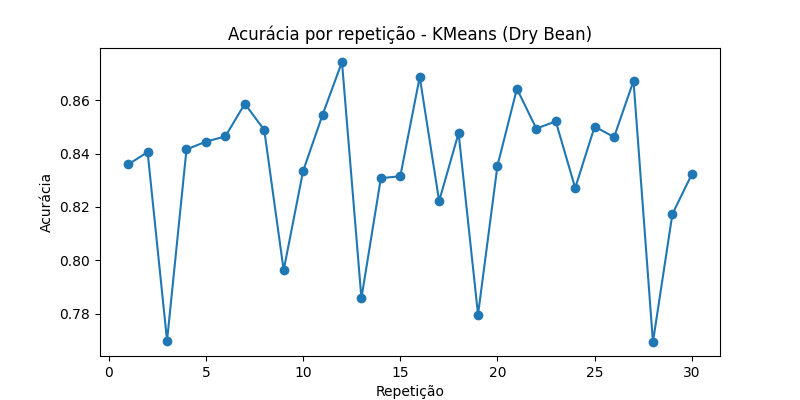
\includegraphics[width=0.9\linewidth]{../src/img/kmeans_drybean_accuracy_repetitions.png}
    \caption{Acurácia por repetição do KMeans no Dry Bean.}
    \label{fig:kmeans_drybean_acc_repeticoes}
\end{figure}

\begin{figure}[ht]
    \centering
    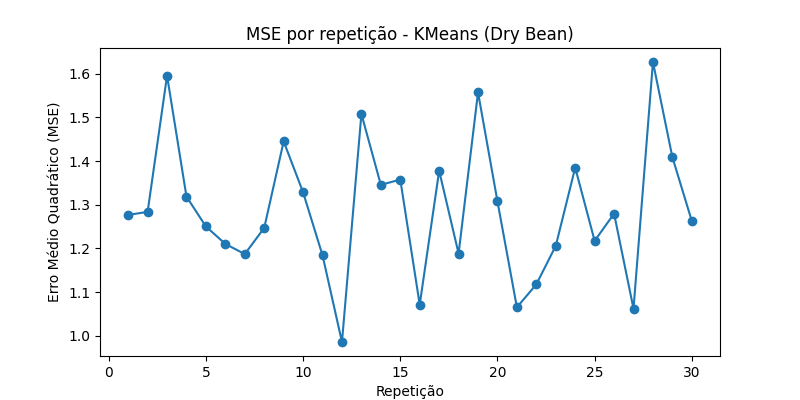
\includegraphics[width=0.9\linewidth]{../src/img/kmeans_drybean_mse_repetitions.png}
    \caption{Erro médio quadrático (MSE) por repetição no Dry Bean.}
    \label{fig:kmeans_drybean_mse_repeticoes}
\end{figure}

% \begin{figure}[ht]
%     \centering
%     \includegraphics[width=0.9\linewidth]{../src/img/kmeans_drybean_confusion_matrix_media.png}
%     \caption{Matriz de confusão média das execuções no Dry Bean.}
%     \label{fig:kmeans_drybean_cm_media}
% \end{figure}

\textbf{Discussão:}

Os resultados mostram que o KMeans supervisionado é capaz de identificar padrões relevantes tanto em problemas binários (Adult) quanto multiclasse (Dry Bean), desde que o pré-processamento e a escolha do número de clusters sejam adequados. No Adult, o balanceamento das classes foi fundamental para evitar viés, enquanto no Dry Bean a distribuição natural das classes já era satisfatória. A análise das métricas e das matrizes de confusão revela que o desempenho do KMeans é consistente ao longo das execuções, mas pode ser impactado pela sobreposição entre classes e pela escolha dos parâmetros iniciais. Recomenda-se, para trabalhos futuros, comparar com outros métodos e explorar técnicas de inicialização e ajuste fino dos hiperparâmetros.

\subsection{Fuzzy C-Means}

% Descrever setup de teste, parâmetros, divisão dos dados, resultados e análise para Fuzzy C-Means

\subsection{Gustafson-Kessel}

% Descrever setup de teste, parâmetros, divisão dos dados, resultados e análise para Gustafson-Kessel
